\chapter{Testing}
\label{chap:test}

This project followed a Behaviour Driven Development (BDD) style from Sprint 3 for the server, and scenario driven GUI testing on the client. In this chapter, I discuss the procedure and the depth of testing in detail.

\section{Server Test}

As discussed in Section \ref{sec:testing}, comprehensive unit testing on the server for each function proved to be a large overhead to a prototyping project, even though agile SE dictates self-contained testing during development sprints. As a result, a more lenient and user-story-driven approach, BDD was used in the project. The format sits between integration and unit testing, but geared more towards the former. Each subsequent sprint also went through a comprehensive round of regression testing. Because the server's main purpose is to provide for a RESTful API, the routes for the API have been tested with boundary cases. Also, independent automated tests were performed to check the database objects' integrity. 100\% of the REST routes that are exposed to the clients have been tested with automated functions given boundary conditions. Each test is self-contained because it creates a sandbox where the  necessary objects are instantiated and cleaned up after success/fail. No external library except the development code was injected into the test suites. However, no granular unit testing was performed, which is necessary in a future production ready server, but avoidable for this short project.

\subsection{REST API Test}

The RESTful API exposes the routes about the User, Thing and Offer objects to the client. For example: a user story may be about borrowing an item. Thus, the route for borrowing is tested so that - users can only borrow a \textit{borrowable} item which is \textit{not closed}, not owned by \textit{himself} etc. The result can be considered a \textit{behaviour} given the \textit{condition}. So, a test is performed for \textit{each} such conditions that may appear on the client side. Figure \ref{fig:rest-test} is the comprehensive list of the tests.\\

As seen in the figure, the tests are easily readable. These tests can be used (and \textit{was} in this project) in the sprint review to negotiate with the customer to \textit{accept} a user-story. For example: the unavoidable unreliability of GCM led me to accept the user-story about push notification, even though the test to expect a notification within 10 seconds would randomly fail.

\begin{figure}[!h]
    \centering
    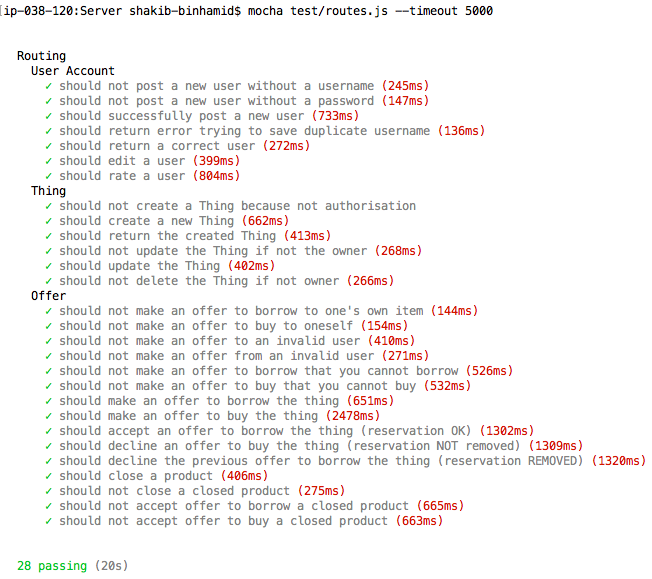
\includegraphics[height = \textwidth, width=\textwidth, keepaspectratio]{routes-test}
    \caption{REST API Behaviour Test}
    \label{fig:rest-test}
\end{figure}

\subsection{Database Integrity Test}

These tests go through each object (\textit{document} in this case) in the database. It then validates the referenced objects and constraints on their fields. For example: in Figure \ref{fig:db-test}, a test fails to find a reservation for a Thing, an offer/request for which was accepted. It means that the offer that it was reserved to is \textit{missing} and the Thing needs to be mended. Note that the actual \textit{fixing} is \textit{not} automated, rather I used these tests to monitor the database.

\begin{figure}[!h]
    \centering
    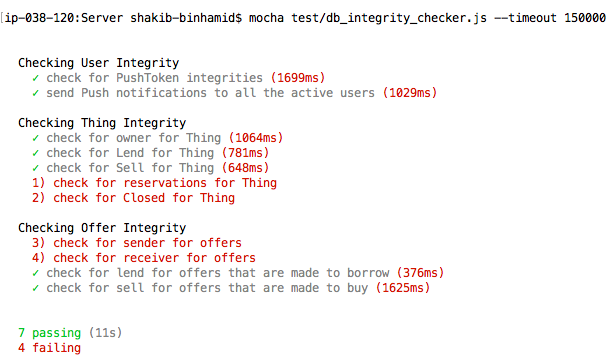
\includegraphics[height = \textwidth, width=\textwidth, keepaspectratio]{db-check}
    \caption{DB Integrity Check}
    \label{fig:db-test}
\end{figure}

\begin{figure}[!h]
    \centering
    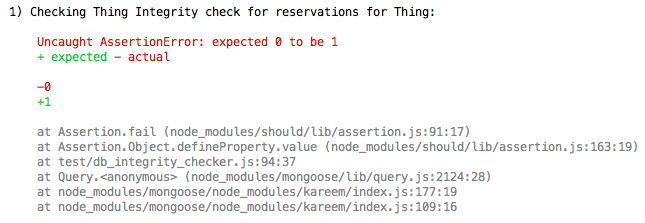
\includegraphics[height = \textwidth, width=\textwidth, keepaspectratio]{error}
    \caption{Error in Testing}
    \label{fig:error}
\end{figure}

The database integrity tests were also performed each sprint. In fact, these tests proved to be so helpful, that I ran them atleast once a development day. I imagine the tests to pave a path to future monitoring mechanism that may be put in place.\\

\section{Client Test}

It was not possible to make automated GUI tests for the client app for the following reasons - 

\begin{itemize}
	\item Touch-event mocking is not possible in Ionic
	\item Ionic libraries cannot be isolated
	\item AngularJS can usually be mocked, but Ionic integrates AngularJS, so it cannot be extracted either
\end{itemize}

In short, BDD or TDD is not possible, because the Ionic framework does not support such features. Even the community is silent in this regard. In fact, as discussed in Chapter \ref{chap:lit} in detail, this is a common problem across mobile app development, specially hybrid apps. I believe the reasons are - 

\begin{itemize}
	\item Ionic is undergoing a complete overhaul for version 2. So, the developers are mostly ignoring the current version.
	\item The production hybrid apps have proprietary, in-house test environments such as in Facebook etc.
\end{itemize}

As a result, I tested the client app regularly against pre-defined set of use case scenarios during development and with end users during UX evaluation.

\subsection{GUI Testing}

To test the GUI, I have exhaustively listed all the use case scenarios in Appendix \ref{appendix:gui-test}. This was built up as each feature had been added. At every sprint, I walked through every scenario multiple times, on two different Android mobiles - Moto X 1st Gen and Moto X Play. I used the list as my primary guide in client app testing. The list is comparable to a 100\% coverage of BDD testing on client.


\subsection{User Evaluation}

I have also evaluated the client app with the end users. More about this is discussed in Chapter \ref{chap:user}, Appendix \ref{appendix:interview} and \ref{appendix:ux}.